%极坐标系

\pentry{平面直角坐标系, 矢量}
\begin{figure}[ht]
\centering
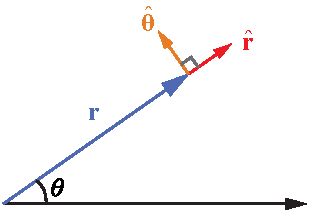
\includegraphics[width=5.2cm]{./figures/Polar1.pdf}
\caption{极坐标系和两个单位矢量}
\end{figure}

在平面上上取一个点作为原点, 过原点作一条轴称为\bb{极轴}, 并选定极轴的正方向,规定单位长度. 该平面上某点与原点连成的线段叫做\bb{极径}, 其长度一般用 $r$ (或 $\rho$ )表示.若 $r$ 为负值, 则表示反方向的长度. 极径与极轴的夹角叫做极角(规定逆时针旋转极角增加,顺时针旋转则减少),用 $\theta $ 表示. $\theta$ 的值通常表示成弧度. 于是任何一点都可以用两个有序实数 $(r,\theta)$ 来表示其在该平面上的位置,这就是一个点的\bb{极坐标}.

为了表示一个坐标对应的单位矢量, 我们一般把坐标变量名记为粗体并在上方加一个标记. 例如直角坐标系中, $\uvec x, \uvec y, \uvec z$ (有时也记为 $\uvec i, \uvec j, \uvec k$ )代表 $x,y,z$ 轴方向的单位矢量. 在极坐标中, 定义 $\uvec r$ 为 $r$ 增加的方向的单位矢量, $\uvec \theta$ 为 $\theta$ 坐标增加方向的单位矢量(即 $\uvec r$ 逆时针旋转 $\pi/2$ 的方向). $\uvec r$ 与 $\uvec \theta$ 互相垂直,构成一对\bb{单位正交基底},平面上的任意矢量都可以正交分解到这两个方向上. 我们通常把 $\uvec r$ 的方向叫做\bb{径向},把 $\uvec \theta $ 的方向叫做\bb{法向}. 要注意极坐标中的两个单位矢量是 $\theta$ 的函数, 对于不同的 $\theta$, 它们的方向也不同.

\begin{exer}{}
试证明极坐标方程 $r = r_0/\cos(\theta - \theta_0)$ 和 $r = 2R\cos(\theta - \theta_0)$ 分别表示一条直线和一个圆.
\end{exer}

\subsection{与直角坐标的转换}
要在极坐标系的基础上建立一个直角坐标系, 习惯的做法是取原点相同, 且令 $x$ 轴与极轴重合, $y$ 轴取 $\theta = \pi/2$ 的方向. 这样将 $\vec r$ 用 $\uvec x$ 和 $\uvec y$ 展开, 就得到
\begin{equation}
\vec r = r\cos\theta\,\uvec x + r\sin\theta\,\uvec y
\end{equation}
即
\begin{equation}\label{Polar_eq2}
\leftgroup{
x &= r\cos\theta\\
y &= r\sin\theta}
\end{equation}
这样就从极坐标转换成为直角坐标.

要从直角坐标转换为极坐标, 首先由勾股定理有 $r^2 = x^2 + y^2$. 使用反正切函数, 我们可以表示 $x >0$ 或 $\theta\in(-\pi/2,\pi/2)$ 时的 $\theta$, 即 $\theta = \arctan(y/x)$. 为了表示任意情况, 本书定义一个值域为 $(-\pi, \pi]$ 的新函数 $\Arctan(y,x)$, 可以把直角坐标中除原点外的任意一点对应的极角表示出来. 这个函数可以用 $\arctan$ 函数定义如下
\begin{equation}
\Arctan(y,x) \equiv 
\leftgroup{
&\arctan (y/x) &\quad &(x > 0)\\
&\arctan (y/x) + \pi  &&(x < 0,\,y \ges 0)\\
&\arctan (y/x) - \pi  &&(x < 0,\,y < 0)\\
&\pi /2  &&(x = 0, \,y > 0)\\
& -\pi /2  &&(x = 0, \,y < 0)\\
&\text{无定义} && (x=0,\,y=0)
}
\end{equation}
这样, 从直角坐标转到极坐标的转换就可以表示为
\begin{equation}\label{Polar_eq4}
\leftgroup{
r &= \sqrt{x^2 + y^2}\\
\theta &= \Arctan(y, x)
}\end{equation}
